\section{Quantum Computing 101}




\begin{frame}{Quantum States}
%	\framesubtitle{The proof uses \textit{reductio ad absurdum}.}



\begin{columns}%[onlywidth,T]
	\begin{column}{.4\textwidth}
\[
\def\arraystretch{1.15}
\underbrace{\scalebox{2}{$\ket{\phi}$}}_{n \text{ qubit state}}
~~~~~=~
\left.
\begin{bmatrix*}[c]
    \frac{i+1}{\sqrt 6} \\ 0 \\ 0 \\ 0\\ \vdots \\0\\ \frac1{\sqrt 3} \\ 0 \\\frac1{\sqrt 3} 
\end{bmatrix*}
~~\right \}\text{$2^n$-sized vector}
\]  
	\end{column}
%\pause
	\begin{column}{.6\textwidth}
\vspace{3mm}\[
\def\arraystretch{1.2}
\scalebox{1.}{$\ket{00\dots01}$}
~=~
\begin{bmatrix*}[c]
    0 \\ 1 \\ 0 \\ 0\\ \vdots \\0\\ 0  \\ 0 \\ 0 
\end{bmatrix*}
\begin{matrix*}[c]
	{\text{$\leftarrow$ index \scriptsize 00\dots00 }} \\ 
	{\text{$\leftarrow$ index \scriptsize 00\dots01 }} \\ \\ \\ \\ \\ \\ \\  
	{\text{$\leftarrow$ index \scriptsize 11\dots10 }} \\  
	{\text{$\leftarrow$ index \scriptsize 11\dots11 }} \\ 
\end{matrix*}
\]  	
	\end{column}
\end{columns}
\pause
\begin{columns}%[onlywidth,T]
	\begin{column}{1\textwidth}
\[
\def\arraystretch{.9}
\scalebox{2}{$\ket{\phi}^\dagger$}
~~=~~
\scalebox{2}{$\bra{\phi}$}
~~=~~
\underbrace{
\begin{bmatrix*}[c]
    \frac{\alert -i+1}{\sqrt 6} ,& 0 ,& 0 ,& 0,& \dots ,&0,&  \frac1{\sqrt 3} ,& 0 ,& 0 ,& \frac1{\sqrt 3} 
\end{bmatrix*}
}_{\text{$2^n$-sized vector (\alert{conjugated} and transposed)}}
\]  
	\end{column}
\end{columns}

\pause

  	\begin{block}{Normalization}
		For $\ket{\phi} =  \begin{bmatrix}\alpha_1, \alpha_2, \dots, \alpha_{n-1}, \alpha_n\end{bmatrix}^T$, we have that $\sum |\alpha_i| = 1$.
		
		~\\
		Or alternatively: $\braket{b|\phi} = \bra{b}\cdot \ket{\phi} = 1$.
  	\end{block}


%  	\begin{block}{Alternative interpretation as pseudo-Boolean function}
%%  		\begin{itemize}
%%  			\item 
%  			A pseudo-Boolean function $f_\phi \colon \set{0,1}^n \to \complex$ such that $f(b) = \braket{b|\phi} = \bra{b}\cdot \ket{\phi}$.
%%  			\\
%%  			~\\
%%  			Here $\bra{b}$ for $b \in \set{0,1}^n$ is a (conjugated) computational basis state, e.g.: $\bra{01} = \begin{bmatrix}0, 0, 0, 0\end{bmatrix}$.
%%  		\end{itemize}
%  	\end{block}


\end{frame}



\begin{frame}{Reversible computing (still classical)}

%\scriptsize
\centering

A circuit computing $(a\land b) \lor c$:

\scalebox{.7}{
\begin{circuitikz}
\draw
(0,2) node[and port] (myand) {\hspace{-1ex}$\land$}
(2,1) node[or port] (myor) {\hspace{-1ex}$\lor$}
(myand.in 1) node[anchor=east] {$a$}
(myand.in 2) node[anchor=east] (bnode) {$b$}
(myand.out) -| node[above]{$x$} (myor.in 1)
node[below=.638cm of bnode] (cnode) {$c$}
(cnode) -|  (myor.in 2)
(myor.out) node[anchor=west] {$y$}
;
\end{circuitikz}
}

How to compute $a,b,c$ given $y$?


\pause

\begin{minipage}{6cm}
\Qcircuit @C=2.em @R=.2em @!R  {
& \lstick{a} & \ctrl{1} & \qw  & \qw      & \qw \\
& \lstick{b} & \ctrl{2} & \qw  & \qw		 & \qw \\
& \lstick{c} & \qw      & \qw  & \ctrl{1} & \qw &\\
& \lstick{x = x_0} & \gate{\land}& \qw&\ctrl{1} & \qw &\rstick{ a\land b}   \\
& \lstick{y = y_0} & \qw      & \qw  & \gate{\lor}&\qw &\rstick{  x\lor c} \\
}
\end{minipage}

\pause
But how to revert the value of $x_0$ and $y_0$?

\pause

\begin{minipage}{6cm}
\Qcircuit @C=2.em @R=.5em @!R  {
& \lstick{a} & \multigate{1}{\land} & \qw  & \qw      & \qw \\
& \lstick{b} & \ghost{\land}  & \qw  & \qw		 & \qw \\
& \lstick{c} & \qw  & \qw  & \multigate{1}{\lor} & \qw &\\
& \lstick{x\alert{=0}} & \targ \qwx[-2] & \qw&\ghost{\land}  & \qw     &\rstick{ x \oplus (a\land b)}  \\
& \lstick{y\alert{=0}} & \qw      & \qw  & \targ \qwx[-1] &\qw &\rstick{y \oplus (x\lor c)} \\
}
\end{minipage}

~\\
\alert{XOR ($\oplus$) is invertible on one input:
$(x\oplus a)\oplus a = x\oplus (a\oplus a) = x$}


\end{frame}



\begin{frame}{Uncomputing reversible computations}

%\scriptsize

\vfill


For any function $f\colon \bool^k \to \bool$, the gate~~~
\begin{minipage}{1cm}
\Qcircuit @C=1em @R=.7em {
&{/}\qw 	& \gate{f} 		& \qw & \qw\\
&\qw  	& \targ\qwx[-1]	& \qw & \qw \\
}
\end{minipage}
~~~is its own inverse!

\pause
\vfill

\hspace{2.5cm}\begin{minipage}{8cm}
\only<1>{
\Qcircuit @C=2.em @R=.5em @!R  {
 \lstick{a} & \multigate{1}{\land} 	& \qw  		& \qw
 			\\
 \lstick{b} & \ghost{\land}        	& \qw		& \qw 
 			\\
 \lstick{c} & \qw    				& \multigate{1}{\lor} & \qw 
 			\\
 \lstick{x{=0}} &\targ \qwx[-2]	&\ghost{\land} & \qw 			
 			&\rstick{ x \oplus ( a\land b)}  \\
 \lstick{o{=0}} & \qw     & \targ \qwx[-1] &\qw 				
 			&\rstick{ o \oplus ( x\lor c)} \\
}
}
\only<+>{
\Qcircuit @C=2.em @R=.5em @!R  {
 \lstick{a} & \multigate{1}{\land} 	& \qw  		& \qw			& \qw & \qw
 			\\
 \lstick{b} & \ghost{\land}        	& \qw		& \qw 			& \qw & \qw
 			\\
 \lstick{c} & \qw    				& \multigate{1}{\lor} & \qw & \multigate{1}{\lor}& \qw
 			\\
 \lstick{x{=0}} &\targ \qwx[-2]	&\ghost{\land} & \qw 			& \ghost{\land}& \qw 
 			&\rstick{ x\oplus ( a\land b)}  \\
 \lstick{o{=0}} & \qw     & \targ \qwx[-1] &\qw 				& \targ \qwx[-1]& \qw
 			&\rstick{  o \oplus ( x\lor c) \oplus ( x\lor c) \alert{= 0}  } \\
}
}
\only<+->{
\Qcircuit @C=2.em @R=.5em @!R  {
 \lstick{a} & \multigate{1}{\land} 	& \qw  		& \qw			& \qw 				& \multigate{1}{\land}& \qw
 			\\
 \lstick{b} & \ghost{\land}        	& \qw		& \qw 			& \qw 				& \ghost{\land} & \qw
 			\\
 \lstick{c} & \qw    				& \multigate{1}{\lor} & \qw & \multigate{1}{\lor}& \qw& \qw
 			\\
 \lstick{x{=0}} &\targ \qwx[-2]	&\ghost{\land} & \qw 			& \ghost{\land}		& \targ \qwx[-2]& \qw
 			&\rstick{  \alert{0} }  \\
 \lstick{o{=0}} & \qw     & \targ \qwx[-1] &\qw 				& \targ \qwx[-1]	& \qw& \qw
 			&\rstick{ \alert{0}} \\
}
\vfill 

~\\
\hspace{-1cm}\alert{To uncomputate, we invert the gate order!}
}
\end{minipage}

\vfill 

\centering

\onslide<+->{
\begin{minipage}{6cm}
\Qcircuit @C=2.em @R=.5em @!R  {
 \lstick{a} & \multigate{1}{\land} 	& \qw  		& \qw						& \multigate{1}{\land}& \qw
 			\\
 \lstick{b} & \ghost{\land}        	& \qw		& \qw 							& \ghost{\land} & \qw
 			\\
 \lstick{c} & \qw    				& \multigate{1}{\lor} & \qw & \qw& \qw
 			\\
 \lstick{x{=0}} &\targ \qwx[-2]	&\ghost{\land} & \qw 				& \targ \qwx[-2]& \qw
 			&\rstick{  {0} }  \\
 \lstick{o{=0}} & \qw     & \targ \qwx[-1] &\qw 					& \qw& \qw
 			&\rstick{ {ab \lor c} \leftarrow \text{cannot uncompute}} \\
}
\end{minipage}
}

\onslide<+->{
\alert{Now to uncompute ${ab \lor c}$, we need to first recompute ${ab}$ }
}


\vfill

\pause
	\textsc{\footnotesize [Landauer (1961)]~~~~~~~~~~~~~~~[Bennett (1973) Logical reversibility of computing]}

\end{frame}



\begin{frame}{Reversible space and time}
	
	
	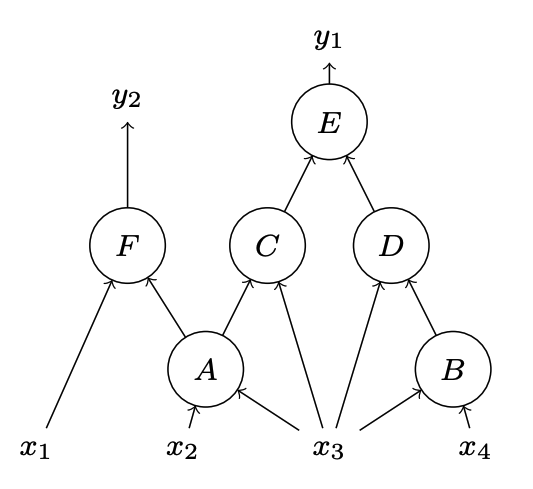
\includegraphics[height=3.cm]{ms1}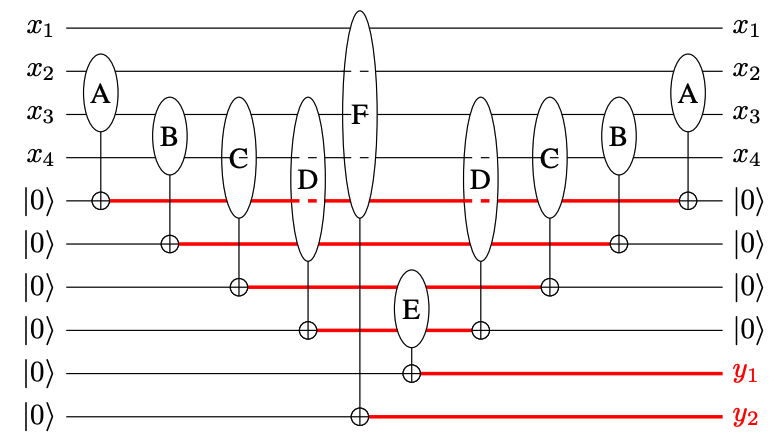
\includegraphics[height=3.5cm]{ms2}
	\raisebox{1.7cm}{\begin{minipage}{1cm}
			$\left . \crule[white]{0cm}{2.5em} \right \}$inputs  \\
			$\left . \crule[white]{0cm}{2.5em} \right \}$ancillas\\
			$\left . \crule[white]{0cm}{1em} \right \}$outputs
			\end{minipage}
	}

\centering 
\onslide<2->{
Do we need one bit per gate?~~~~~~~ Expensive: Space = Time.
}

\onslide<3->{
	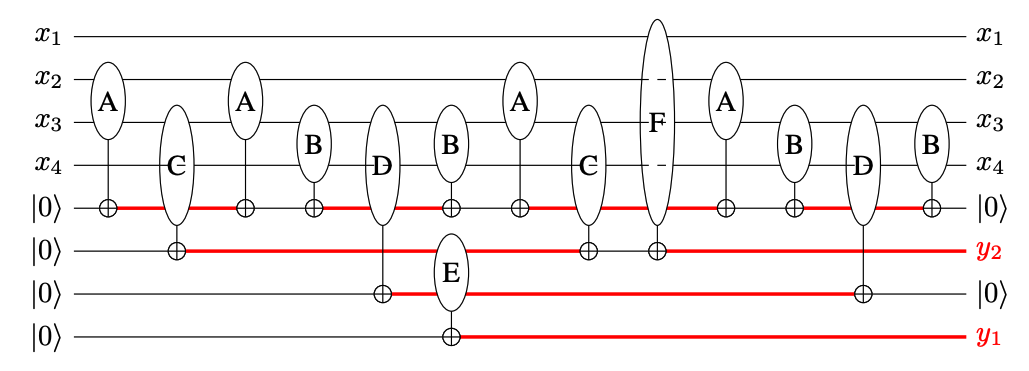
\includegraphics[height=3.cm]{ms3}
}

	\vspace{-1em}
	\textsc{\footnotesize [Meuli et al. (2019) Reversible Pebbling Game for Quantum Memory Management]}

\end{frame}



\begin{frame}{Reversible Circuit Evaluation with Matrices}


\begin{exampleblock}{One-qubit case}

\begin{columns}
\begin{column}{.2\textwidth}
A one bit circuit:\\\vspace{2ex}
\hspace{1em}\Qcircuit @C=1em @R=.7em {
\lstick 0  	& \gate{\neg} 		& \qw & \rstick 1 \\
%\lstick 0   	& \targ\qwx[-1]	& \qw & \qw \\
}
\end{column}
%\begin{column}{.15\textwidth}
%	\tab{0 \\ 1 } \mat{a\\b}
%\end{column}
\begin{column}{.3\textwidth}
\pause
.. with \textit{vectors as states}:\\\vspace{2ex}
~\phantom{ZZZZZ}\Qcircuit @C=1em @R=.7em {
\lstick{\mat{1\\0}}  	& \gate{\neg} 		& \qw & \rstick{\mat{0\\1}} \\
%\lstick 0   	& \targ\qwx[-1]	& \qw & \qw \\
}
\end{column}
\begin{column}{.3\textwidth}
.. not ($\neg$) is a matrix:\\\vspace{1ex}
$X = \mat{0 & 1\\ 1 & 0}$
\end{column}
\end{columns}


\vspace{2em}

\pause
\begin{columns}
\begin{column}{.45\textwidth}
So evaluation becomes matrix-vector multiplication:\\
~
\end{column}
\begin{column}{.45\textwidth}
$\underbrace{\mat{0& 1\\ 1 & 0}}_{X}\cdot \mat{1\\ 0} =  \mat{0\\ 1}$
\end{column}
%\begin{column}{.25\textwidth}
%$\underbrace{\mat{1& 1\\ 1 & 1}}_{?}\cdot \mat{1\\ 0} =  \mat{1\\ 1}$
%\end{column}
\end{columns}



\vspace{1ex}
\vspace{1ex}
\vspace{1ex}
\pause

\alert{We read circuits from left to right, but the linear algebra works the other way around!}

\begin{align*}
\hspace{1em}\Qcircuit @C=1em @R=.7em {
\lstick{\mat{1\\0}}  	& \gate{A} & \gate{B} & \gate{C} 		& \qw & 
%\lstick 0   	& \targ\qwx[-1]	& \qw & \qw \\
}
=   C\cdot B \cdot A \cdot \mat{1\\0}
\end{align*}


\vspace{1ex}
\end{exampleblock}

	
\end{frame}




\begin{frame}{Reversible Circuit Evaluation with Matrices}

\begin{exampleblock}{Multi-qubit case}

\begin{columns}
\begin{column}{.24\textwidth}
\hspace{1em}Three-bit circuit:\\\vspace{2ex}
\hspace{2.5em}\Qcircuit @C=1em @R=.7em {
\lstick 1  	& \multigate{1}{\land}	& \qw & \rstick 1 \\
\lstick 1  	& \ghost{\land}			& \qw & \rstick 1 \\
\lstick 0   & \targ\qwx[-1]			& \qw & \rstick 1 \\
}
\end{column}
\begin{column}{.34\textwidth}
States become vectors..\\\vspace{1ex}
{$ \ket{110} = \smat{0 \\ 0 \\ 0 \\ 0 \\ 0 \\ 0 \\ 1 \\ 0 }\ket{111} = \smat{0 \\ 0 \\ 0 \\ 0 \\ 0 \\ 0 \\ 0 \\ 1 }$}
\end{column}
\begin{column}{.4\textwidth}
.. Tofolli gate becomes a matrix:\\\vspace{1ex}
$CCX = \smat{1 & 0 & 0 & 0 & 0 & 0 & 0 & 0 \\
			0 & 1 & 0 & 0 & 0 & 0 & 0 & 0 \\
			0 & 0 & 1 & 0 & 0 & 0 & 0 & 0 \\
			0 & 0 & 0 & 1 & 0 & 0 & 0 & 0 \\
			0 & 0 & 0 & 0 & 1 & 0 & 0 & 0 \\
			0 & 0 & 0 & 0 & 0 & 1 & 0 & 0 \\
			0 & 0 & 0 & 0 & 0 & 0 & \alert 0 & \alert 1 \\
			0 & 0 & 0 & 0 & 0 & 0 & \alert 1 & \alert 0 \\}$
\end{column}
\end{columns}


\vspace{2em}

\pause
\begin{columns}
\begin{column}{.2\textwidth}
As matrix-vector multiplication:\\
~
\end{column}
\begin{column}{.7\textwidth}
$CCX \cdot \ket{110} = \smat{1 & 0 & 0 & 0 & 0 & 0 & 0 & 0 \\
			0 & 1 & 0 & 0 & 0 & 0 & 0 & 0 \\
			0 & 0 & 1 & 0 & 0 & 0 & 0 & 0 \\
			0 & 0 & 0 & 1 & 0 & 0 & 0 & 0 \\
			0 & 0 & 0 & 0 & 1 & 0 & 0 & 0 \\
			0 & 0 & 0 & 0 & 0 & 1 & 0 & 0 \\
			0 & 0 & 0 & 0 & 0 & 0 & \alert 0 & \alert 1 \\
			0 & 0 & 0 & 0 & 0 & 0 & \alert 1 & \alert 0 \\} \cdot   \smat{0 \\ 0 \\ 0 \\ 0 \\ 0 \\ 0 \\ 1 \\ 0 } =  \smat{0 \\ 0 \\ 0 \\ 0 \\ 0 \\ 0 \\ 0 \\ 1} =  \ket{111}$
\end{column}
\end{columns}


\vspace{1ex}
\end{exampleblock}

\pause
\centering
\alert{Overkill to compute with exponentially sized vectors?}
	
\end{frame}




\begin{frame}{Superpositions}

\begin{exampleblock}{Adding superpositions}
\begin{columns}
\begin{column}{.25\textwidth}
A one bit circuit:\\\vspace{1ex}
\hspace{1em}\Qcircuit @C=1em @R=.7em {
\lstick 0  	& \gate{X} 		& \qw & \rstick 1 \\
%\lstick 0   	& \targ\qwx[-1]	& \qw & \qw \\
}
\end{column}
%\begin{column}{.15\textwidth}
%	\tab{0 \\ 1 } \mat{a\\b}
%\end{column}
\begin{column}{.3\textwidth}
\pause
 .. a `normal' operation:\\\vspace{1ex}
\hspace{1em}\Qcircuit @C=1em @R=.7em {
\lstick{\mat{1\\0}}  	& \gate{X} 		& \qw & \rstick{\mat{0\\1}} \\
%\lstick 0   	& \targ\qwx[-1]	& \qw & \qw \\
}

\end{column}
\begin{column}{.25\textwidth}
\pause
 .. superposition op.:\\\vspace{1ex}
\hspace{1em}
\Qcircuit @C=1em @R=.7em {
\lstick{\mat{1\\0}} 	& \gate{?} 		& \qw & \rstick{\mat{1\\1}} \\
%\lstick 0   	& \targ\qwx[-1]	& \qw & \qw \\
}
\end{column}
\end{columns}

\vspace{2em}

\pause
\begin{columns}
\begin{column}{.2\textwidth}
In linear algebra:\\
~
\end{column}
\begin{column}{.25\textwidth}
$\underbrace{\mat{0& 1\\ 1 & 0}}_{X}\cdot \mat{1\\ 0} =  \mat{0\\ 1}$
\end{column}
\begin{column}{.25\textwidth}
$\underbrace{\mat{1& 1\\ 1 & 1}}_{?}\cdot \mat{1\\ 0} =  \mat{1\\ 1}$
\end{column}
\end{columns}



\vspace{1ex}
\vspace{1ex}
\vspace{1ex}

\vspace{1ex}
\end{exampleblock}


\pause
\begin{alertblock}{Two problems}
\begin{enumerate}
	\item How to make this \alert{reversible}? We have:
$\mat{1& 1\\ 1 & 1}\cdot \alert{\mat{1\\ 0}} =  \mat{1& 1\\ 1 & 1}\cdot 
   \alert{\mat{0\\ 1}} =  \mat{1\\ 1}$
\pause
	\item What does the state \mat{1\\1} mean? Non-determinism? Parallelism? Probability?
\end{enumerate}
\end{alertblock}

\end{frame}




\begin{frame}{Superpositions and reversibility}

\begin{exampleblock}{Making superpositions reversible with a \alert{Hadamard gate}}


Define $\alert H = \nicefrac1{\sqrt 2}  \mat{1& 1\\ 1 & -1}$.

\pause
Note that $H\cdot H = 
%		\nicefrac1{\sqrt 2}  \mat{1& 1\\ 1 & -1} \cdot
%		\nicefrac1{\sqrt 2}  \mat{1& 1\\ 1 & -1} =
		\nicefrac12 \mat{2& 0\\ 0 & 2} = \mat{1& 0\\ 0 & 1} = \id$,
so we have \alert{reversibility:}
~\\

\begin{align*}
\Qcircuit @C=1em @R=.7em {
\lstick{\mat{a\\b}} 	& \gate{H} 		& \gate{H} 	 & \qw & \rstick{\hspace{-1em} \mat{a\\b }} & \\
%\lstick 0   	& \targ\qwx[-1]	& \qw & \qw \\
} 
~~=~~
\Qcircuit @C=1em @R=.7em {
&&\lstick{\mat{a\\b}} 	& \gate{\id}	 & \qw & \rstick{\hspace{-1em} \mat{a\\b }} & \\
%\lstick 0   	& \targ\qwx[-1]	& \qw & \qw \\
}
~~=~~
\Qcircuit @C=1em @R=.7em {
&&\lstick{\mat{a\\b}} 	& \qw & \qw & \qw & \rstick{\hspace{-1em} \mat{a\\b }} \\
%\lstick 0   	& \targ\qwx[-1]	& \qw & \qw \\
}
\end{align*}

~\\
~\\

\pause

\vspace{2ex}
\begin{columns}
\begin{column}{.1\textwidth}
\end{column}
\begin{column}{.4\textwidth}
From `basis state' 0:\\\vspace{2ex}
\hspace{1em} \Qcircuit @C=1em @R=.7em {
\lstick{\mat{1\\0}} 	& \gate{H} 		& \qw & \rstick{\hspace{-1em} \frac1{\sqrt 2} \mat{1\\1}} \\
%\lstick 0   	& \targ\qwx[-1]	& \qw & \qw \\
}
\end{column}
\begin{column}{.4\textwidth}
From `basis state' 1:\\\vspace{2ex}
\hspace{1em}
\Qcircuit @C=1em @R=.7em {
\lstick{\mat{0\\1}} 	& \gate{H} 		& \qw & \rstick{\hspace{-1em}\frac1{\sqrt 2} \mat{1\\-1}} \\
%\lstick 0   	& \targ\qwx[-1]	& \qw & \qw \\
}
\end{column}
\end{columns}

\vspace{2em}

\pause
\begin{columns}
\begin{column}{.02\textwidth}
%In linear algebra:
\end{column}
\begin{column}{.4\textwidth}
$\frac1{\sqrt 2}\mat{1& 1\\ 1 & -1}\cdot \mat{1\\ 0} =  \frac1{\sqrt 2}\mat{1\\ 1}$
\end{column}
\begin{column}{.4\textwidth}
$\frac1{\sqrt 2}\mat{1& 1\\ 1 & -1}\cdot \mat{0\\ 1} = \frac1{\sqrt 2} \mat{1\\ -1}$
\end{column}
\end{columns}


\vspace{1.5em}

\vspace{1ex}
\end{exampleblock}


\end{frame}




\begin{frame}{Superpositions on the superbit plane}


\centering



%\begin{textblock}{6}(.5,.3)
%\only<2->{
	\begin{tikzpicture}[scale=1.9,cap=round,>=latex,font=\scriptsize]

        \draw[-] (1.5cm,0cm) -- (-1.5cm,0cm) node[left,fill=white]
        {\hphantom{$x \text{(basis state 0)} $}};

        % draw the coordinates
        \draw[->] (-1.5cm,0cm) -- (1.5cm,0cm) node[right,fill=white] {$x \text{(basis state 0)} $};
        \draw[->] (0cm,-1.5cm) -- (0cm,1.5cm) node[above,fill=white] {$y \text{(basis state 1)}$};



        % draw the unit circle
        \draw[thick] (0cm,0cm) circle(1cm);

        \foreach \x /\y  [evaluate=\y as \xtext using 180/\y]
          in {45} {
                % lines from center to point
                \draw[gray] (0cm,0cm) -- (\x:1cm);
                \draw[dotted] (0.71cm,0cm) -- node[left] {$\frac 1{\sqrt2}$} (\x:1cm);
                \draw[dotted] (0cm,0.71cm) -- node[above left] {$\frac 1{\sqrt2}$} (\x:1cm);
                % dots at each point
                \filldraw[black] (\x:1cm) circle(0.4pt);
                % draw each angle in degrees
                
                \draw (\x:1.45cm) node[fill=white] (a) {\mat{\nicefrac1{\sqrt2}\\ \nicefrac1{\sqrt2}} };
                
%              \draw[gray] (0cm,0cm) -- (-\x:1cm);              
%
%                \draw[dotted] (0.71cm,0cm) -- node[left] {$\frac 1{\sqrt2}$} (-\x:1cm);
%                \draw[dotted] (0cm,-0.71cm) -- node[above left] {$\frac 1{\sqrt2}$} (-\x:1cm);
%                
%%                \draw (\x:0.6cm) node[fill=white] {$\x^\circ$};
%                \draw (-\x:1.45cm) node[fill=white] (a) {\mat{\nicefrac1{\sqrt2}\\ -\nicefrac1{\sqrt2}} };
%%                \draw (\x:0.6cm) node[fill=white] {$\frac{\pi}{4}$};
        }

        \draw (-1.3cm,0cm) node[above=1pt] {$-1$}
              (1.25cm,0cm)  node[above=1pt] {$1$}
              (0.2cm,-1.25cm) node[] {$-1$}
              (0.2cm,1.25cm)  node[] {$1$};
              
%        \draw[bend left=20,->,dotted] (a)  node {} -- (5.2, 1.5);
    \end{tikzpicture}
%}
%\end{textblock}

\pause
\alert{Not the complex plane!}

\end{frame}



\begin{frame}{Superpositions and measurement}

\begin{exampleblock}{Making superpositions readable through \alert{measurement}}


\vspace{1ex}

\begin{columns}
\begin{column}{.1\textwidth}
\end{column}
%\begin{column}{.15\textwidth}
%	\tab{0 \\ 1 } \mat{a\\b}
%\end{column}
\begin{column}{.4\textwidth}
%From `basis state' 0:\\\vspace{2ex}
\hspace{1em} \Qcircuit @C=1em @R=.7em {
\lstick{\mat{1\\0}} 	& \qw 		& \meter &	\rstick{\tab{p(0) = 1 \\ p(1) = 0  }} \\
%\lstick 0   	& \targ\qwx[-1]	& \qw & \qw \\
}
\end{column}
\begin{column}{.4\textwidth}
%From `basis state' 1:\\\vspace{2ex}
\hspace{1em}
\Qcircuit @C=1em @R=.7em {
\lstick{\mat{0\\1}} 	& \qw		&  \meter &	\rstick{\tab{p(0) = 0\\ p(1) = 1  }}
%\lstick 0   	& \targ\qwx[-1]	& \qw & \qw \\
}
\end{column}
\end{columns}

\pause
\vspace{5ex}


\begin{columns}
\begin{column}{.1\textwidth}
\end{column}
%\begin{column}{.15\textwidth}
%	\tab{0 \\ 1 } \mat{a\\b}
%\end{column}
\begin{column}{.4\textwidth}
%From `basis state' 0:\\\vspace{2ex}
\hspace{1em} \Qcircuit @C=1em @R=.7em {
\lstick{\mat{1\\0}} 	& \gate{H} 		& \meter &	\rstick{\tab{p(0) = \nicefrac12 \\ p(1) = \nicefrac12  }} \\
%\lstick 0   	& \targ\qwx[-1]	& \qw & \qw \\
}
\end{column}
\begin{column}{.4\textwidth}
%From `basis state' 1:\\\vspace{2ex}
\hspace{1em}
\Qcircuit @C=1em @R=.7em {
\lstick{\mat{0\\1}} 	& \gate{H} 		&  \meter &	\rstick{\tab{p(0) = \nicefrac12 \\ p(1) = \nicefrac12  }}
%\lstick 0   	& \targ\qwx[-1]	& \qw & \qw \\
}
\end{column}
\end{columns}

\vspace{2em}

\pause

\begin{columns}
\begin{column}{.02\textwidth}
%In linear algebra:
\end{column}
\begin{column}{.4\textwidth}
$\frac1{\sqrt 2}\mat{1& 1\\ 1 & -1}\cdot \mat{1\\ 0} =  \mat{\nicefrac1{\sqrt2}\\ \nicefrac1{\sqrt2}}$
\end{column}
\begin{column}{.4\textwidth}
$\frac1{\sqrt 2}\mat{1& 1\\ 1 & -1}\cdot \mat{0\\ 1} =  \mat{\nicefrac1{\sqrt2}\\ \alert{-\nicefrac1{\sqrt2}}}$
\end{column}
\end{columns}

\pause

\centering
\vspace{1em}




\onslide<+->{}

In general, we have a state \mat{a \\ b}, which \ul{indirectly} represents a \alert{probability distribution:}

\vspace{1ex}
\begin{tabular}{c|c|c}
\bf Old state &	\bf Outcome 			& \onslide<+->{\bf New state} \\\hline
 \mat{a \\ b}  & 0 = \mat{1\\0}	with $p(0) = a^2$ & \onslide<.->{\mat{1\\0}}
  \rule{0cm}{.6cm}
  \\
 \mat{a \\ b}  & 1 = \mat{0\\1}	with $p(1) = b^2$ & \onslide<.->{\mat{0\\1}}	\rule{0cm}{.6cm}
\end{tabular}

\vspace{1ex}
\vspace{1ex}

\onslide<.->{
\alert{State collapses after measurement to measurement outcome!}
}

\vspace{1ex}
\end{exampleblock}


\end{frame}




\begin{frame}{Quantum State Representation with the
					\alert{Stabilizer Formalism}}

Pauli gates:~~~~ $I = \mat{1&0\\0&1},~~~~X = \mat{0&1\\1&0} ~~~~Y = \mat{0&-i\\i&0}~~~~Z = \mat{1&0\\0&-1}$

\begin{exampleblock}<2->{Stabilizing single-qubit states}

\begin{itemize}
	\item 
All single-qubit states $\ket{\phi}$ are stabilized by $\mathbb{I}$, because $I \cdot \ket{\phi}= \ket{\phi}$.

\item ~~$Z \cdot \ket{0} = \mat{1&0\\0&-1} \cdot \mat{1\\0} = \mat{1\\0} = \ket 0$
\item $-Z \cdot \ket{1} = \mat{-1&0\\0&1} \cdot \mat{0\\1} = \mat{0\\1} = \ket 1$
\pause
\item
\only<+>{ ~~$P \cdot \ket{+} = ~~P \cdot \mat{1\\1} = \mat{1\\1} = \ket +$ for which $P \in \set{\mathbb{I}, X, Y, Z}$?}
\pause
 ~~$X \cdot \ket{+} = ~~X \cdot \mat{1\\1} = \mat{1\\1} = \ket +$ 
\pause
\item
 $-X \cdot \ket{-} = ~~X \cdot \mat{1\\1} = \mat{1\\1} = \ket -$ 
\end{itemize}

\end{exampleblock}



\pause
\begin{exampleblock}{Two-qubit stabilizer states}

\begin{itemize}
	\item  $\ket{00}$ is stabilized by $I \otimes I, Z\otimes I, I\otimes Z$ and $Z\otimes Z$.
	\item The Bell state $
    \ket{\phi} \approx  \ket{00} + \ket{11}
$ is stabilized by $I \otimes I, Z\otimes Z, X\otimes X$ and $-Y\otimes Y$
\end{itemize}

%\begin{columns}
%\begin{column}{.3\textwidth}
%~~~~~~~The Bell state:\\
%~~~~~~$
%    \ket{\phi} \approx  \ket{00} + \ket{11}
%%    \begin{bmatrix*}[c]
%%    1,\\ 0,\\ 0,\\ 1\phantom,\\
%%    \end{bmatrix*}
%$
%\end{column}
%\begin{column}{.18\textwidth}
%\Qcircuit @C=2.3em @R=1.2em {
% & \gate{X} & \qw  \\
%&  \gate{X} & \qw \\ 
%  & \lstick{X \otimes X\hspace{-1cm}} & \dstick{}
%\gategroup{1}{2}{2}{2}{.7em}{--}
%}
%\end{column}
%\begin{column}{.18\textwidth}
%\Qcircuit @C=2.3em @R=1.2em {
% & \gate{Z} & \qw  \\
%&  \gate{Z} & \qw \\
%  & \lstick{Z\otimes Z\hspace{-1cm}} & \dstick{}
%\gategroup{1}{2}{2}{2}{.7em}{--}
%}
%\end{column}
%\begin{column}{.3\textwidth}
%Stabilized by:
%\vspace{3mm}
%
%$
%\ket{\phi} = X \otimes X \cdot \ket { \phi }
%$
%
%$
%\ket{\phi} = Z \otimes Z \cdot \ket { \phi }
%$
%\end{column}
%\end{columns}
\end{exampleblock}

				
\end{frame}	




\begin{frame}{Quantum State Representation with the
					\alert{Stabilizer Formalism}}




\begin{definition}
\begin{itemize}
	\item In general, an $n$-qubit stabilizer state $\ket\phi$ is stabilized by a set $S_\phi$ of $2^n$ stabilizers.

%\centering
\alert{But this is still exponentially sized?!?}

\pause
	\item The set $S_\phi$ forms a group under multiplication.
	
\pause

	\item The group $S_phi$ has generator $G_\phi$ with $n$ elements, i.e., $\gen{G_\phi} = S_\phi$

\pause

\item The generators are referred to as the \alert{(quadratically-sized)} ``stabilizer tableau'':
\[
\begin{bmatrix*}
P_{1,1}~~~ \otimes & P_{1,2}~~~ \otimes & \dots & \otimes~~~ P_{1,n}\\
P_{2,1}~~~ \otimes& P_{2,2}~~~  \otimes& \dots & \otimes~~~ P_{2,n}\\
\vdots  & \vdots  & \ddots& \vdots\\
P_{n,1}~~~ \otimes& P_{n,2}~~~ \otimes & \dots &  \otimes~~~ P_{n,n}\\
\end{bmatrix*} \text{ for } P_{i,j} \in \hspace{-.5em} \underbrace{\set{\id, X, Y, Z}}_{ \text{ single qubit Pauli's}}
\]
\vspace{-1em}
\pause

\item We can obtain the density matrix of $\ket\phi$ from its stabilizer group
\[
\ket{\phi}\hspace{-1mm}\bra{\phi} ~~~~~~~=~~ \underbrace{\frac1{2^n}\cdot \sum_{P \in S_\phi}  P}_{\text{normalized sum of stabilizers}}   \pause ~~~=~~~ \underbrace{\prod_{P\in G_\phi} \frac{(P + I)}2}_{\text{normalized product of generators}}
\]
\vspace{-1em}

\item Applying a (Clifford) gate $U$ to $\ket\phi$ can be done on the stabilizers:
\[
U \cdot \ket{\phi}\hspace{-1mm}\bra{\phi} \cdot U^\dagger ~~~~~~~=~~ {\frac1{2^n}\cdot \sum_{P \in S_\phi}  U \cdot P\cdot U^\dagger}
\]


\end{itemize}
\end{definition}

\pause
\centering
\alert{Used in error correction, etc.}


\end{frame}



